\documentclass{article}
\usepackage[utf8]{inputenc}
\usepackage{graphicx}
\usepackage{amsmath}
\usepackage{amsfonts}
\usepackage[a4paper, margin=1in]{geometry}
\title{Homework 7}
\author{Steve Gillet}
\date{\today}

% Custom information
\newcommand{\className}{Course: Algorithmic Motion Planning – ASEN 5254-001 – Fall 2024}
\newcommand{\professorName}{Professor: Morteza Lahijanian}
\newcommand{\taName}{Teaching Assistant: Yusif Razzaq}

\begin{document}

% Title
\maketitle
\begin{center}
    \large{\className} \\
    \large{\professorName} \\
    \large{\taName}
\end{center}

\section*{Exercise 1.
Implement a simple probabilistic roadmap (PRM) planner that samples \textit{n} configurations 
(before validity check) and connects each valid sample to every valid configuration that is within 
radius \textit{r} from it through a straight line. Assume that the C-space is a rectangle in $\mathbb{R}^2$ 
with \textit{x} $\in$ [$\mathit{x}_{min}$, $\mathit{x}_{max}$] and \textit{y} = [$\mathit{y}_{min}$, $\mathit{y}_{max}$]. 
The program should take \textit{n}, \textit{r}, obstacles, C-space boundaries, and $q_{start}$ and $q_{goal}$ 
as input and return the roadmap, a path from $q_{start}$ to $q_{goal}$, the path length, and the computation time.
}

\subsection*{(a) Solve the planning problem in \textbf{Exercise 2.(a)} of \textbf{Homework 5} with boundaries $\mathit{x} \in [-1, 11]$ and $\mathit{y} = [-3,3]$.}

\subsubsection*{i. Plot the roadmap and the solution path for \textit{n} = 200 and \textit{r} = 1. Indicate the path length in the title of the plot.}

\begin{figure}[h]
    \centering
    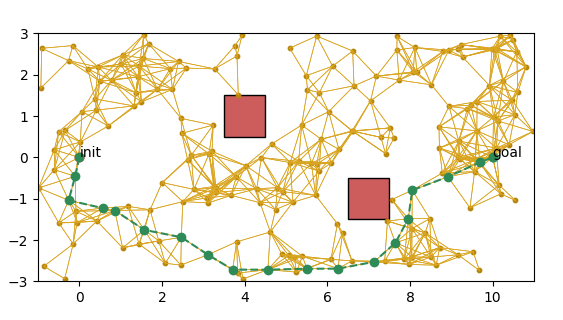
\includegraphics[width=0.8\textwidth]{hw5prmPlot.png}
    \caption{Homework 5 Exercise 2 Problem Plot. Path Length = 13.0364.}
    \label{fig:hw5prmPlot}
\end{figure}

\subsubsection*{ii. Vary $n$ and $r$ and benchmark your solutions in three categories of number of valid solutions, path length, and computation time. For benchmarking, use 100 runs for each
\[
(n, r) \in \{(200, 0.5), (200, 1), (200, 1.5), (200, 2), (500, 0.5), (500, 1), (500, 1.5), (500, 2)\}.
\]
Show your results using boxplots.}

\begin{figure}[h]
    \centering
    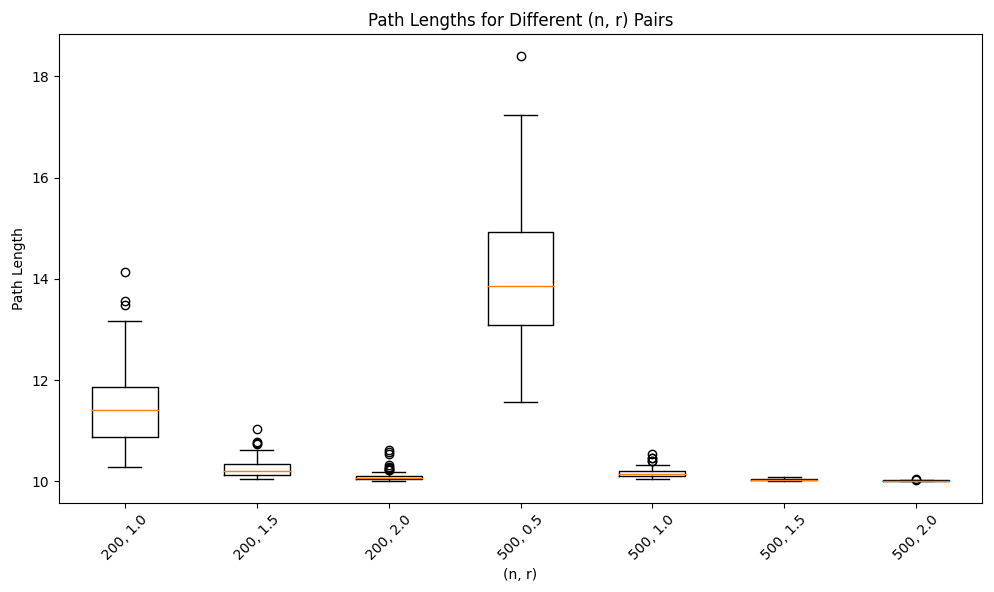
\includegraphics[width=0.8\textwidth]{e1a2pathLengths.png}
    \caption{Box Plot Path Lengths}
    \label{fig:e1a2pathLengths}
\end{figure}

\begin{figure}[h]
    \centering
    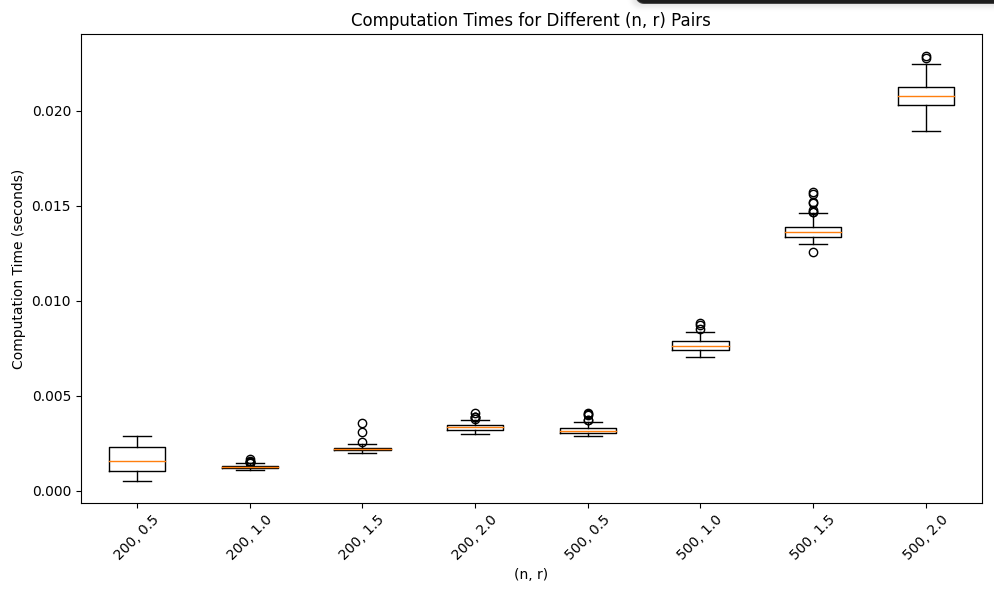
\includegraphics[width=0.8\textwidth]{e1a2times.png}
    \caption{Box Plot Computation Times}
    \label{fig:e1a2times}
\end{figure}

\begin{figure}[h]
    \centering
    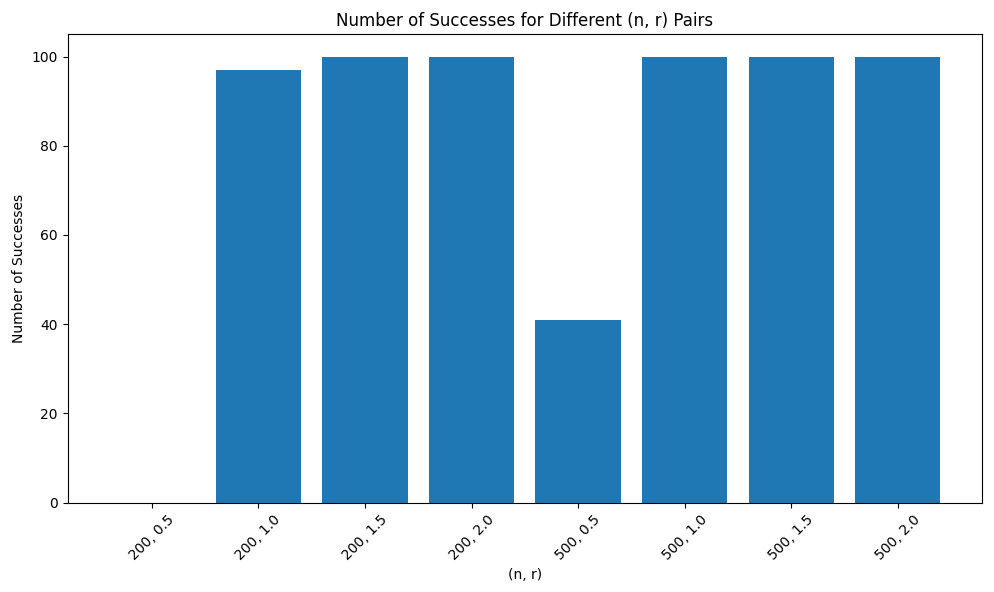
\includegraphics[width=0.8\textwidth]{e1a2successes.png}
    \caption{Bar Graph Successes}
    \label{fig:e1a2successes}
\end{figure}

\subsubsection*{iii. Based on your empirical evaluations, what are the optimal values for \textit{n} and \textit{r}? Justify your answer.} 

I'd say that 200 samples and 2 radius is the ideal just based on my opinion of the results without any actual metric to weigh the importance of the different independent variables.
200 samples, 2 radius gets you just about as effective of a path length as the higher sample rate with much less in terms of computation time and the same success rate.

\subsubsection*{iv. Augment your PRM planner with a path smoothing technique and re-evaluate your bench-
marks. What are the optimal values for \textit{n} and \textit{r} with path smoothing? Justify your answer.}

\begin{figure}[h]
    \centering
    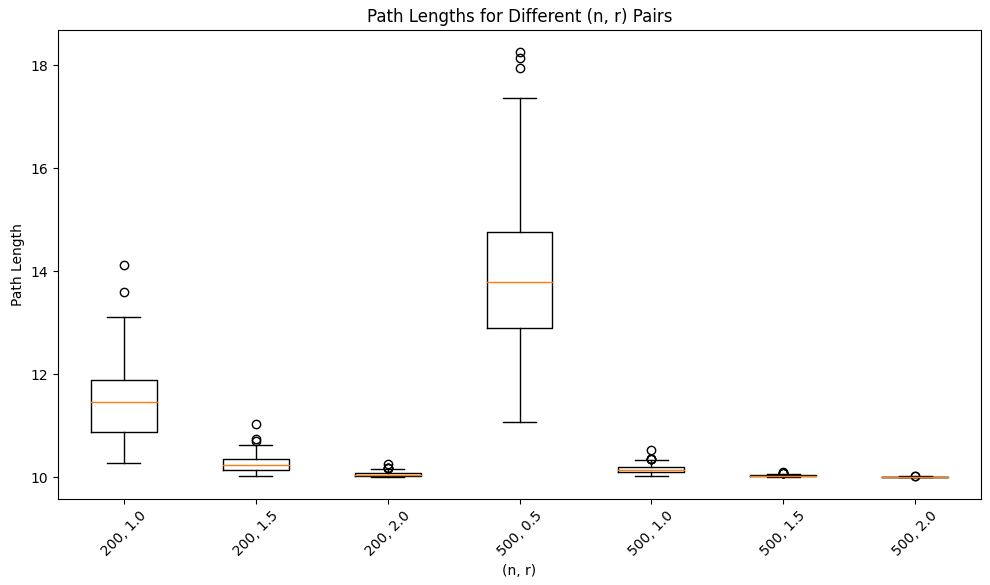
\includegraphics[width=0.8\textwidth]{e1a4pathLengths.png}
    \caption{Box Plot Smoothed Path Lengths}
    \label{fig:e1a4pathLengths}
\end{figure}

\begin{figure}[h]
    \centering
    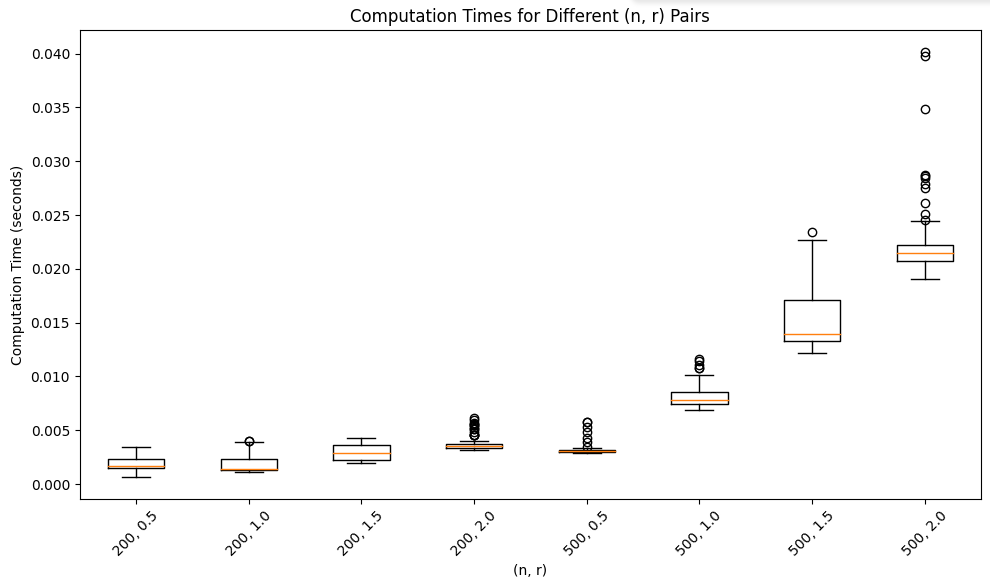
\includegraphics[width=0.8\textwidth]{e1a4times.png}
    \caption{Box Plot Smoothed Successes}
    \label{fig:e1a4times}
\end{figure}

\begin{figure}[h]
    \centering
    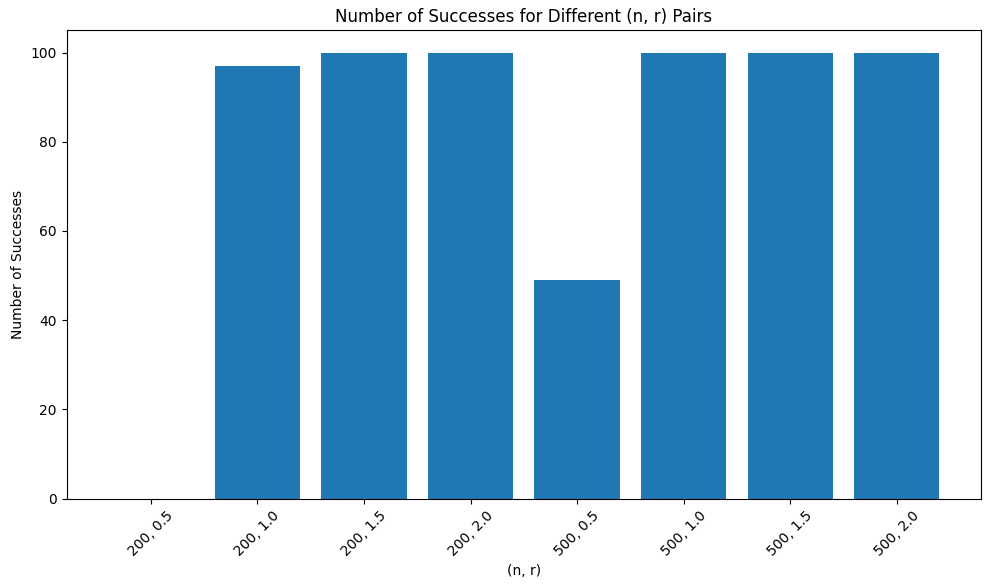
\includegraphics[width=0.8\textwidth]{e1a4successes.png}
    \caption{Bar Graph Smoothed Successes}
    \label{fig:e1a4successes}
\end{figure}

The results show that the path length is basically unchanged and the computation time is increased.
That makes sense to me in this simple environment where the path is always essentially a straight line.
The best \textit{n} and \textit{r} is still 200 and 2 for the same reasons as before the smoothing, the smoothing had very little effect in this case.

\subsection*{(b) Solve the planning problems in \textbf{Exercise 2} of \textbf{Homework 2} using your PRM (no path smoothing). For each $\mathit{W}_1$ and $\mathit{W}_2$, perform the following steps:}

\subsubsection*{i. Plot the roadmap and the solution path for \textit{n} = 200 and \textit{r} = 2. Indicate the path length in the title of the plots.}

\begin{figure}[h]
    \centering
    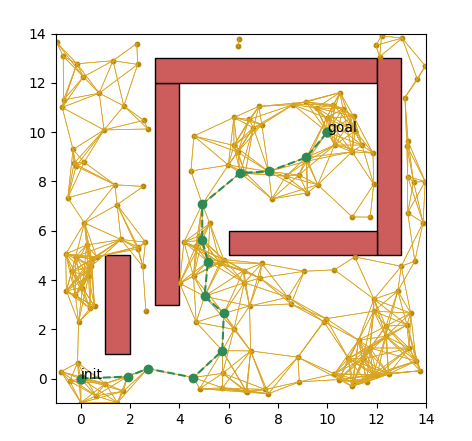
\includegraphics[width=0.8\textwidth]{e1b1plot.png}
    \caption{Homework 2 Exercise 2 Workspace 1 PRM Plot, Path Length: 15.7841}
    \label{fig:e1b1plot}
\end{figure}

\begin{figure}[h]
    \centering
    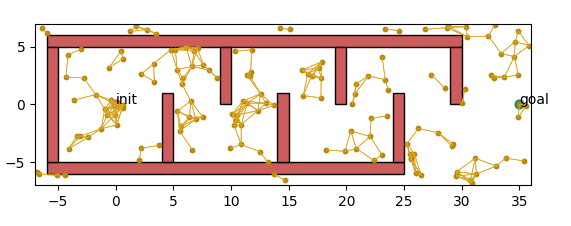
\includegraphics[width=0.8\textwidth]{e1b1w2plot.png}
    \caption{Homework 2 Exercise 2 Workspace 2 PRM Plot, Path Length: 0 (No Valid Path)}
    \label{fig:e1b1w2plot}
\end{figure}

See Figure~\ref{fig:e1b1plot} for Workspace 1 and Figure~\ref{fig:e1b1w2plot} for Workspace 2.

\subsubsection*{ii. Vary $n$ and $r$ and benchmark your solutions in three categories of number of valid solutions, path length, and computation time. For benchmarking, use 100 runs for each
\[
(n, r) \in \{(200, 0.5), (200, 1), (200, 1.5), (200, 2), (500, 0.5), (500, 1), (500, 1.5), (500, 2)\}.
\]
Show your results using boxplots.}

\begin{figure}[h]
    \centering
    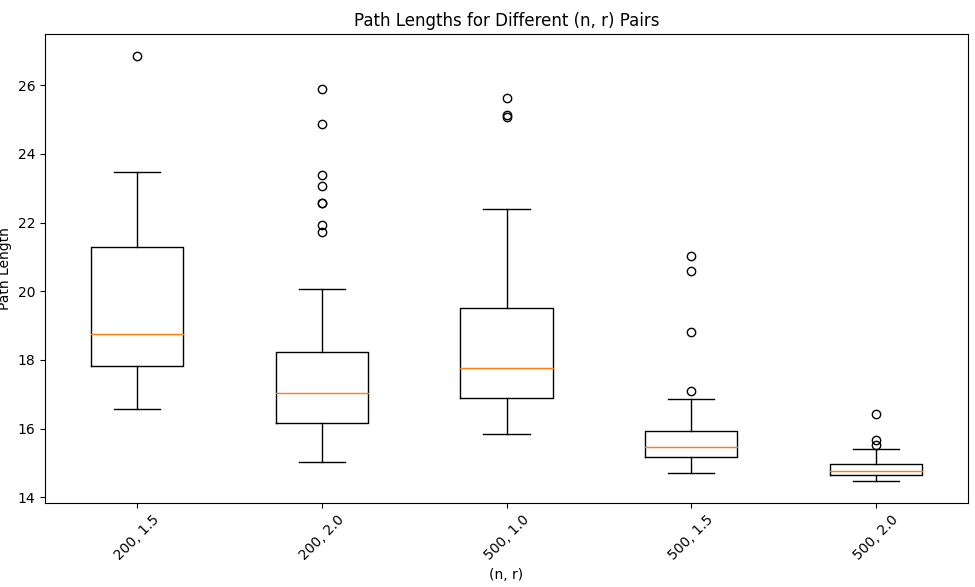
\includegraphics[width=0.8\textwidth]{e1b2w1pathLengths.png}
    \caption{Box Plot Path Lengths Homework 2 Workspace 1}
    \label{fig:e1b2w1pathLengths}
\end{figure}

\begin{figure}[h]
    \centering
    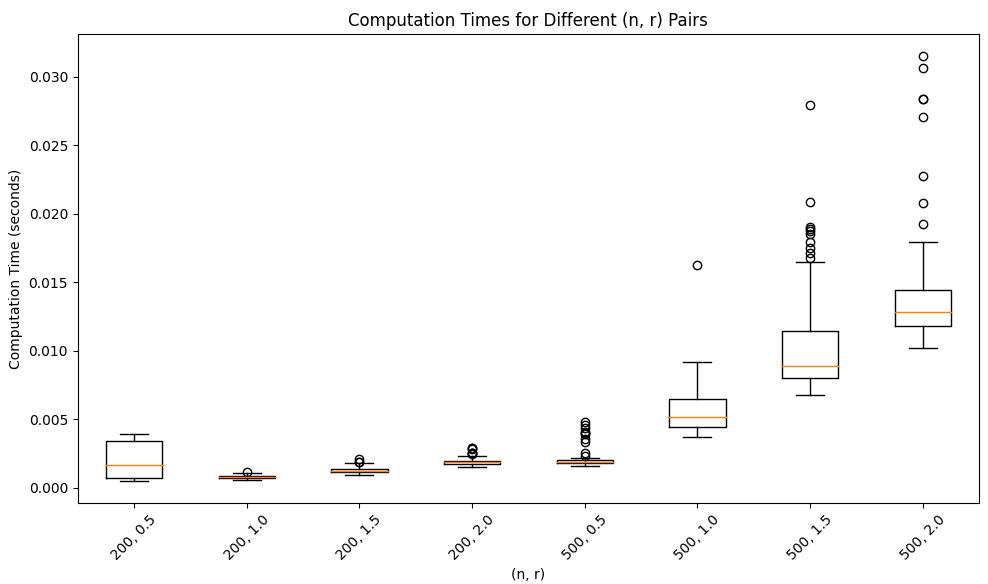
\includegraphics[width=0.8\textwidth]{e1b2w1times.png}
    \caption{Box Plot Computation Times Homework 2 Workspace 1}
    \label{fig:e1b2w1times}
\end{figure}

\begin{figure}[h]
    \centering
    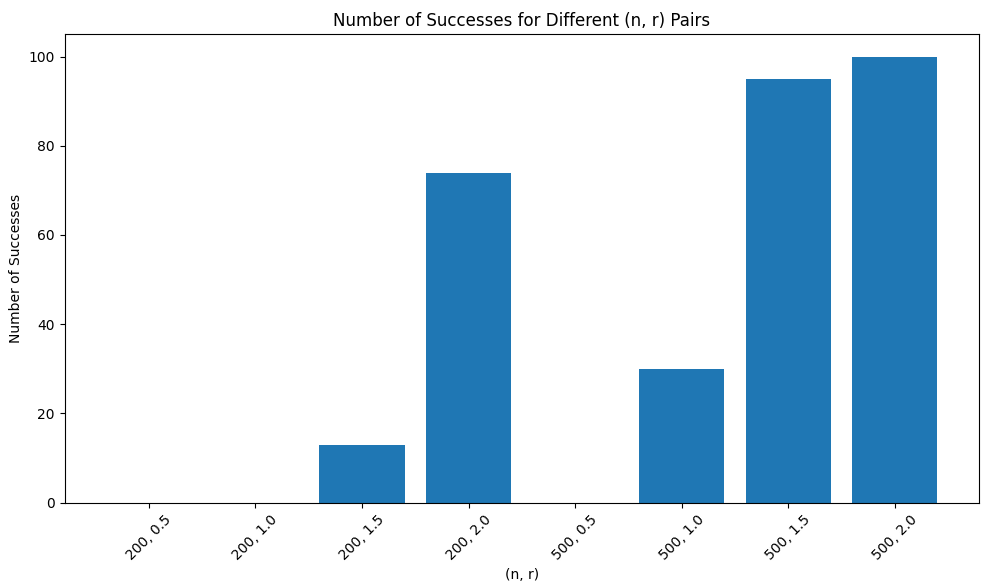
\includegraphics[width=0.8\textwidth]{e1b2w1successes.png}
    \caption{Bar Graph Successes Homework 2 Workspace 1}
    \label{fig:e1b2w1successes}
\end{figure}

\begin{figure}[h]
    \centering
    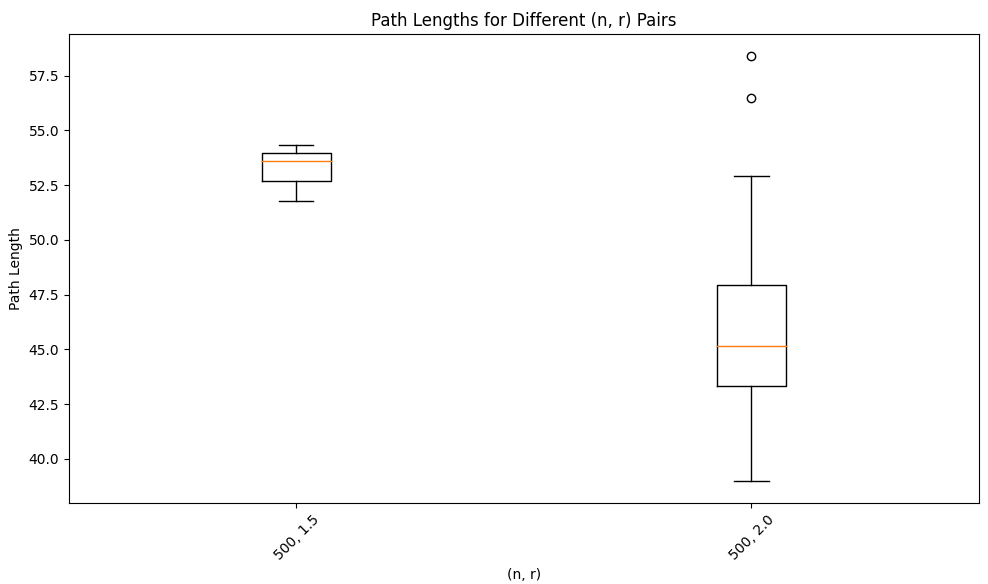
\includegraphics[width=0.8\textwidth]{e1b2w2pathLengths.png}
    \caption{Box Plot Path Lengths Homework 2 Workspace 2}
    \label{fig:e1b2w2pathLengths}
\end{figure}

\begin{figure}[h]
    \centering
    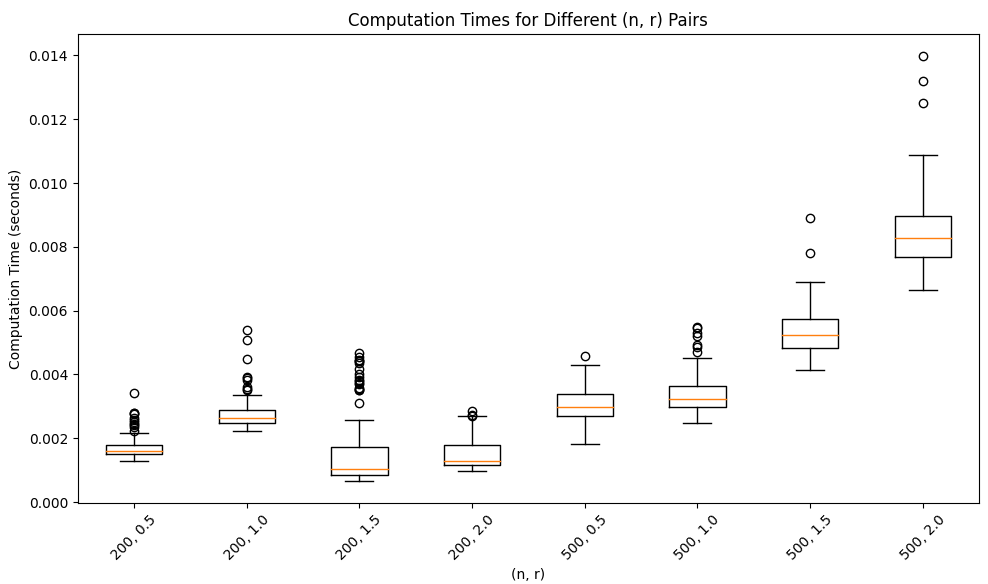
\includegraphics[width=0.8\textwidth]{e1b2w2times.png}
    \caption{Box Plot Computation Times Homework 2 Workspace 2}
    \label{fig:e1b2w2times}
\end{figure}

\begin{figure}[h]
    \centering
    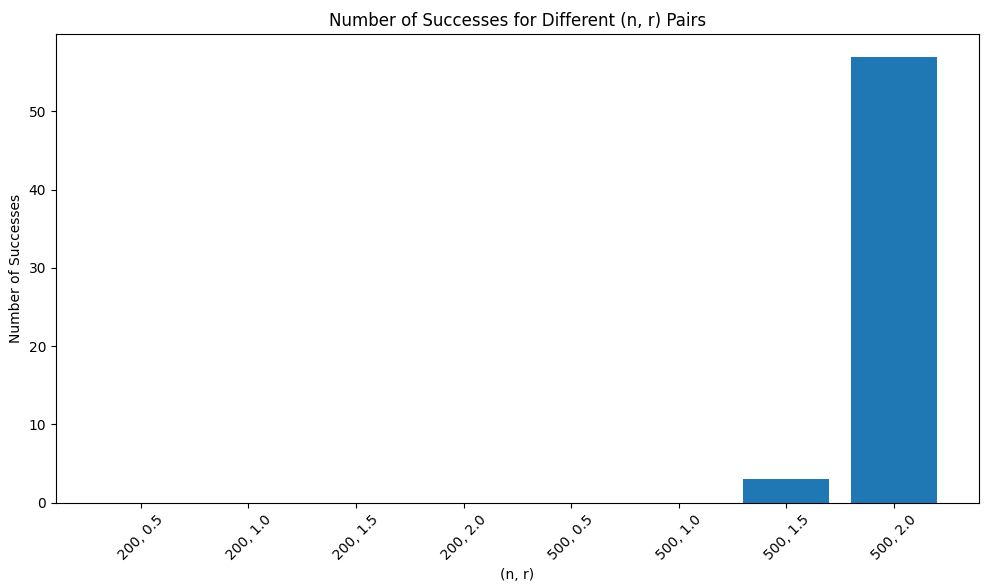
\includegraphics[width=0.8\textwidth]{e1b2w2successes.png}
    \caption{Bar Graph Successes Homework 2 Workspace 2}
    \label{fig:e1b2w2successes}
\end{figure}

See Figures~\ref{fig:e1b2w1pathLengths}, \ref{fig:e1b2w1times}, \ref{fig:e1b2w1successes} for Workspace 1 and Figures~\ref{fig:e1b2w2pathLengths}, \ref{fig:e1b2w2times}, \ref{fig:e1b2w2successes} for Workspace 2.

\subsubsection*{iii. Based on your empirical evaluations, what are the optimal values for \textit{n} and \textit{r} in $\mathit{W}_1$ and $\mathit{W}_2$? Justify your answer.}

Based on empirical evaluations I would say the optimal values for \textit{n} and \textit{r} for Workspace 1 is 500 and 2 because the path length is significally shorter and the success rate is 100\%, the computation time is definitely higher but still pretty small and worth it for the extra success.
For Workspace 2, 500 and 2 is really the only answer. Only 500 and 2 and 500 and 1.5 had any successful paths and 500 and 1.5 only had 3 out of 100. It's a difficult workspace and you just need a lot of samples and radius to get a path.

\subsubsection*{iv. Enable path smoothing option in your PRM and re-evaluate your benchmarks. What are the optimal values for \textit{n} and \textit{r} with path smoothing? Justify your answer.}

Path smoothing reduced the path lengths for all of the values of \textit{n} and \textit{r} and both Workspaces and effected the computation time in about the same way.
I think the optimal values stay the same although path smoothing definitely does help I would still choose 500 and 2.

\subsection*{(c) Does your PRM implementation need to change in order for it to solve the planning problem in Exercise 2 of Homework 6? Justify your answer.}

No, we can apply the same planner to that problem except that we would apply it to the configuration space instead of the workspace. But it would work for the same reasons the wavefront planner that we used in that problem worked.

\section*{Exercise 2.
Implement the basic GoalBiasRRT planner with step size \(r\) and goal bias probability of \(p_{goal}\). Assume that the C-space is a rectangle in \(\mathbb{R}^2\) with \(x \in [x_{min}, x_{max}]\) and \(y \in [y_{min}, y_{max}]\). The program should take \(r\), \(p_{goal}\), maximum number of iterations \(n\), obstacles, C-space boundaries, \(q_{start}\), \(q_{goal}\), and radius \(\epsilon\) (centered at \(q_{goal}\)) for the termination condition at goal as input and return a path from \(q_{start}\) to \(q_{goal}\), the path length, and the computation time.
Solve the planning problems in \textit{Exercise 1.(a)-(b)} using your basic RRT implementation with \(n = 5000\), \(r = 0.5\), \(p_{goal} = 0.05\), and \(\epsilon = 0.25\).
}

\subsection*{(a)
For each environment, plot one solution path and its corresponding tree. Indicate the path length in the title of the plot.
}

\begin{figure}[h]
    \centering
    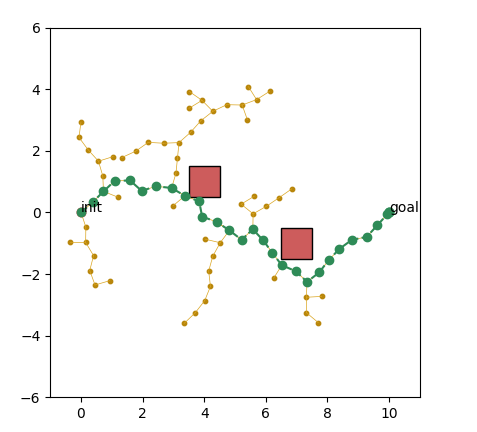
\includegraphics[width=0.8\textwidth]{e2aHW5plot.png}
    \caption{Homework 5 Workspace RRT Plot, Path Length: 13.0745}
    \label{fig:e2aHW5plot}
\end{figure}

For Homework 5 Workspace 1, see Figure~\ref{fig:e2aHW5plot}.

\begin{figure}[h]
    \centering
    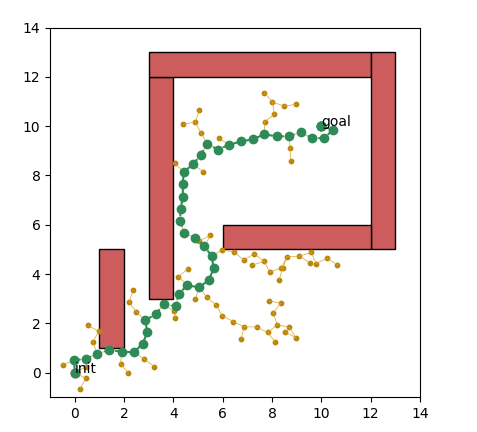
\includegraphics[width=0.8\textwidth]{e2aHW2W1plot.png}
    \caption{Homework 2 Workspace 1 RRT Plot, Path Length: 20.5064}
    \label{fig:e2aHW2W1plot}
\end{figure}

For Homework 2 Workspace 1, see Figure~\ref{fig:e2aHW2W1plot}.

\begin{figure}[h]
    \centering
    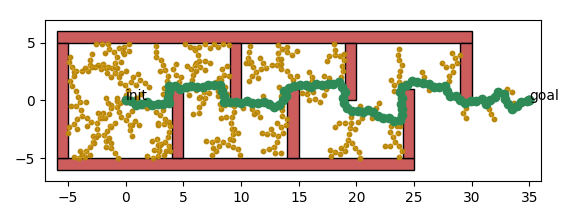
\includegraphics[width=0.8\textwidth]{e2aHW2W2plot.png}
    \caption{Homework 2 Workspace 2 RRT Plot, Path Length: 47.214}
    \label{fig:e2aHW2W2plot}
\end{figure}

For Homework 2 Workspace 2, see Figure~\ref{fig:e2aHW2W2plot}.

\subsection*{(b)
For each environment, use 100 runs to benchmark your implementation in three categories of number of valid solutions, path length, and computation time. Show your results using boxplots.
}

\begin{figure}[h]
    \centering
    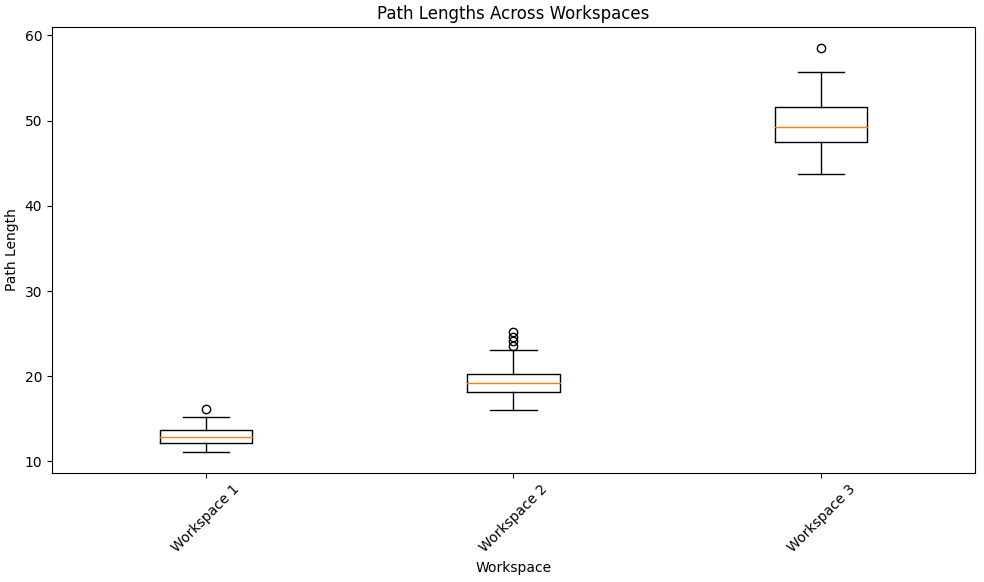
\includegraphics[width=0.8\textwidth]{e2bPathLengths.png}
    \caption{RRT Plot Path Lengths Per Workspace}
    \label{fig:e2bPathLengths}
\end{figure}

For the benchmark path lengths, see Figure~\ref{fig:e2bPathLengths}. Workspace 1 corresponds to Homework 5 Workspace 1, Workspace 2 to Homework 2 Workspace 1, and Workspace 3 to Homework 2 Workspace 2.

\begin{figure}[h]
    \centering
    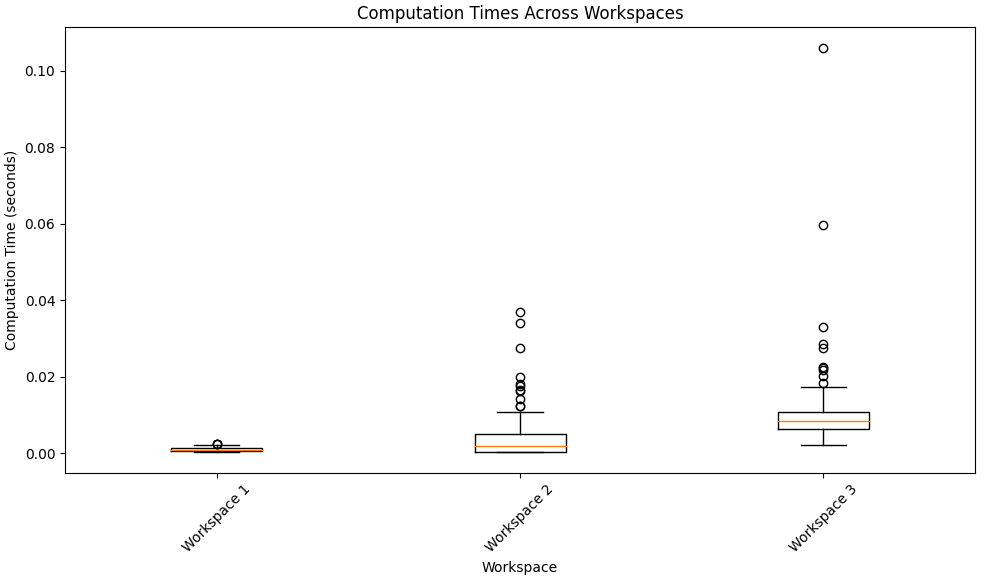
\includegraphics[width=0.8\textwidth]{e2bTimes.png}
    \caption{RRT Plot Computation Times Per Workspace}
    \label{fig:e2bTimes}
\end{figure}

For the benchmark computation times, see Figure~\ref{fig:e2bTimes}.

\begin{figure}[h]
    \centering
    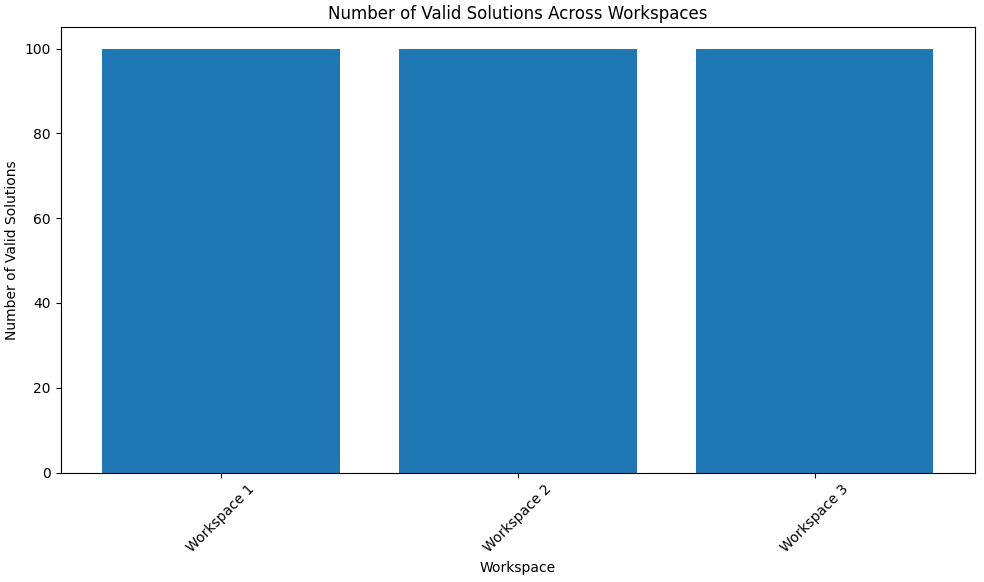
\includegraphics[width=0.8\textwidth]{e2bSuccesses.png}
    \caption{RRT Plot Successes Per Workspace}
    \label{fig:e2bSuccesses}
\end{figure}

For the benchmark computation times, see Figure~\ref{fig:e2bSuccesses}.

\subsection*{(c)
Does your RRT implementation need to change in order for it to solve the planning problem in \textit{Exercise 2 of Homework 6}? Justify your answer.
}

Again no, not really. You would just use the same planner on the c-space instead of the workspace. You might want to change the distance metric since in the c-space it might not make sense to just use Euclidean distance but the planner works the same way.

\section*{Exercise 3
You have implemented four planners (gradient descent with a potential function, wavefront, PRM, and RRT) to solve planning problems in \textit{Exercise 2.(a)-(c)}. Reflect on the performance of these planners and provide a discussion on their advantages and disadvantages.
}

Gradient descent was the most difficult to implement and probably the least effective because of local minima and the large amount of tuning required for the different parameters.
I like gradient descent and think it's cool and perhaps if I had more time to play with it I would improve it to the point where it would be more effective.

Wavefront was easier to implement than gradient descent, still a bit challenging. But really effective once you dial it in. Obviously you can't apply it to every problem, especially high dimension problems but it is very efficient.

PRM was the easiest to implement by far and pretty effective frankly especially with smoothing you basically get the most optimal path in a relatively short period of time.

RRT was slightly more difficult to implement but definitely way easier than gradient descent or wavefront and it was remarkably good at finding a path and finding it quickly.
I think the way it was biased towards the goal just meant that it would quickly move out in that direction and in some cases almost just go directly there.
Very impressive and I think if you added smoothing you would have something that is the fastest and effectively as close to optimal as the others or close enough.

\end{document}
